%!TEX program = xelatex
\documentclass[11pt,a4paper]{article}
\usepackage{polyglossia}
\usepackage[autostyle=true]{csquotes}
\setdefaultlanguage{italian}
\usepackage{listings}
\usepackage{graphicx}
\usepackage{caption}
\lstset{language=VHDL,
    columns=flexible,
    basicstyle={\small\ttfamily},
    numbers=left}
\title{\textbf{Progetto di Reti Logiche 2020}}
\author{Tomas Antonio Lopez}
\begin{document}

\maketitle
\tableofcontents
\listoffigures

\newpage

\section{Introduzione}
Il componente richiesto consiste in un \emph{working-zone encoder} per indirizzi a 7 bit, con output a 8 bit.\\
Al primo segnale di \emph{start} dopo un \emph{reset}, il componente carica la lista di indirizzi base delle working-zones dalla memoria, disposte
secondo la specifica fornita, e produce in uscita l'indirizzo letto in input, eventualmente codificato come richiesto. Un successivo segnale di
\emph{start} porta il dispositivo a riutilizzare le working-zones precedentemente caricate per codificare il nuovo indirizzo in input. Nel caso in cui
dovesse giungere un segnale di \emph{reset} durante qualunque stadio della computazione, lo stato del dispositivo verrebbe reinizializzato e,
successivamente, le working-zones ricaricate qualora un segnale \emph{start} alto dovesse venir rilevato.\\
Si assume che il segnale di \emph{reset} proveniente dall'esterno sia opprtunamente filtrato e privo di glitch.

\section{Architettura}
\begin{figure}[ht]
    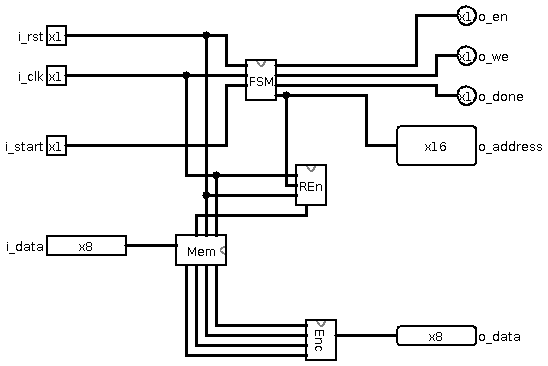
\includegraphics[scale=0.65]{component.png}
    \caption[Il componente]{Architettura del componente.}
\end{figure}

Architetturalmente, il componente è composto da due blocchi funzionali:
\begin{itemize}
    \item un controller sequenziale, che si occupa del trasferimento dei dati dalla RAM esterna alle memorie di lavoro interne e della scrittura del
        risultato in RAM, nonché dell'invio dei segnali di controllo appropriati;
    \item un encoder puramente combinatorio, che produce in uscita l'indirizzo, eventualmente codificato, basandosi sul contenuto delle memorie
        interne.
\end{itemize}
Durante la progettazione si è cercato di ridurre al minimo la presenza di elementi \emph{stateful} per evitare di incorrere in problemi di
sincronizzazione o reset incompleti. Inoltre, essendo l'encoder composto da circuiti combinatori, la velocità di conversione è sufficientemente alta da
permettere al componente di concludere le operazioni nel giro di 3 cicli di clock, quando le working-zones sono già presenti nella memoria di lavoro.

\subsection{Memoria di lavoro}
\begin{figure}[htp]
    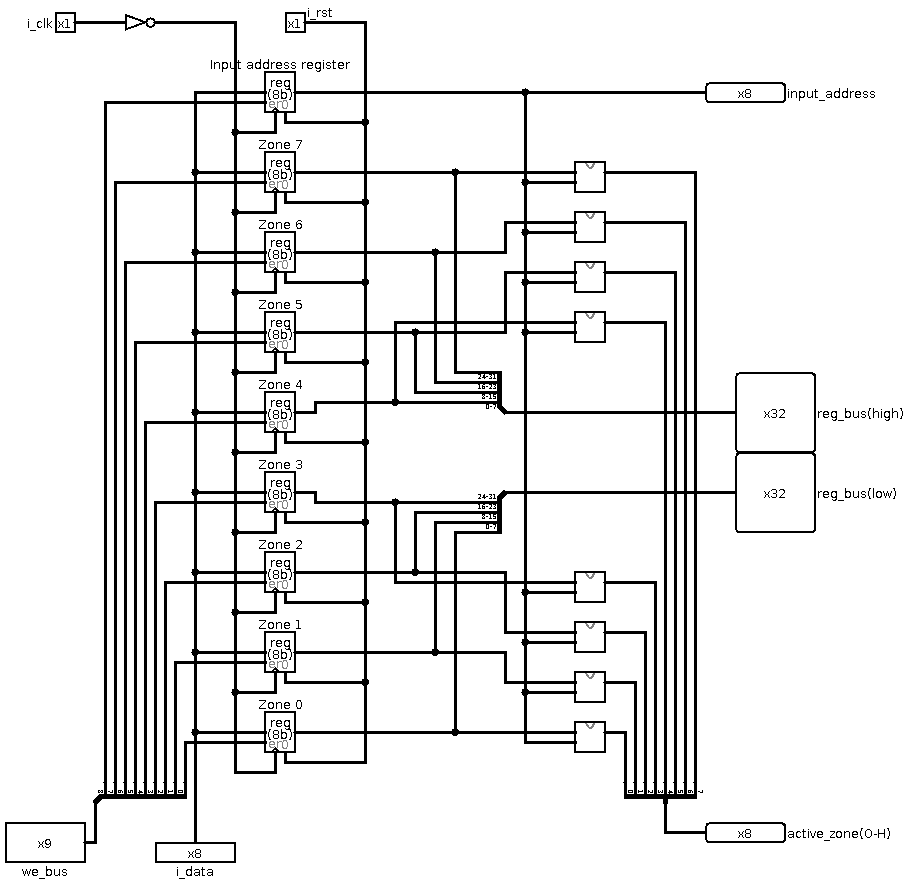
\includegraphics[scale=0.39]{memories.png}
    \caption[Memorie e comparatori]{Il banco di registri, assieme ai comparatori paralleli.}
\end{figure}

Il componente è dotato di un banco di 9 registri PIPO a reset asincrono da 8 bit, contenente gli indirizzi base delle working-zones e l'indirizzo da
codificare. Tutti i registri sono collegati ad un bus comune che ne controlla il segnale di \emph{write-enable} (\lstinline{we_bus}), sono direttamente
connessi con la porta di reset globale (\lstinline{i_rst}) e funzionano a clock inverso.

Il trigger è stato posto sul fronte di discesa perché la RAM esterna produce i nuovi output sul fronte di salita. In questo modo, è possibile memorizzare i
dati di lavoro non appena disponibili, senza ulteriore orchestrazione da parte dell'unità di controllo.

\subsection{Encoder}
\begin{figure}[htp]
    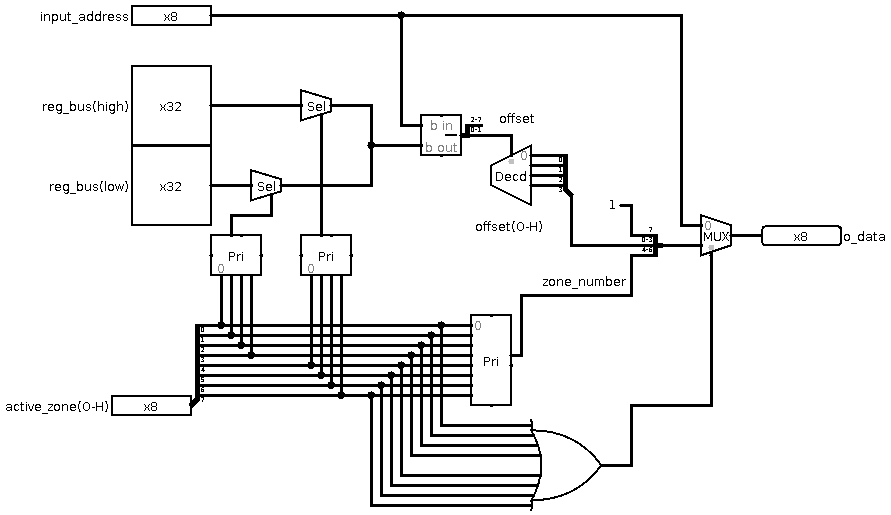
\includegraphics[scale=0.4]{encoder.png}
    \caption[Encoder]{L'encoder combinatorio.}
\end{figure}

\begin{figure}[hp]
    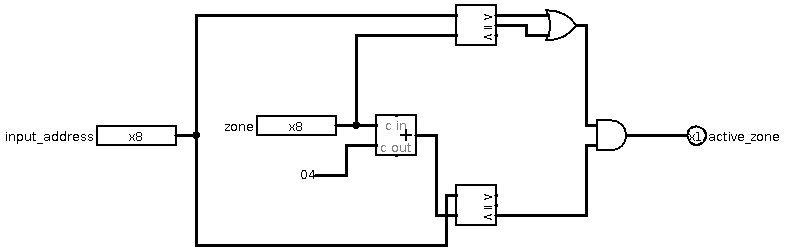
\includegraphics[scale=0.4]{comparator.png}
    \caption[Comparatore]{Schema di una unità comparatrice.\label{comparator}}
\end{figure}

L'encoder si collega direttamente alle memorie contenenti le basi delle working-zones\footnote{In realtà, i comparatori sono strettamente integrati con i
registri di lavoro. Dal punto di vista del linguaggio di descrizione, infatti, fanno parte dello stesso modulo.} e ne dirige l'output verso 8 comparatori
paralleli [\ref{comparator}].
Tali comparatori verificano se l'indirizzo da codificare (memorizzato sul nono registro) cade all'interno della working-zone di propria competenza. Nel
caso in cui ciò dovesse accadere, il comparatore della working-zone valida segnalerebbe sul bus \lstinline{active_zone} la propria attivazione.

In seguito all'eventuale attivazione di una working-zone, un encoder ed un selettore si occupano di transcodificare il numero della working-zone attiva
da one-hot a binario e di prelevare il suo indirizzo base, rispettivamente. L'indirizzo base viene poi portato agli ingressi di un sottrattore, che
calcola l'offset dell'indirizzo da codificare rispetto alla base.

Infine, l'offset viene decodificato in one-hot e concatenato all'altro sottocampo e al bit addizionale.

Nel caso in cui nessuna working-zone dovesse risultare attiva, un semplice multiplexer devia l'indirizzo ricevuto in input direttamente verso l'output.

\subsection{Controller}
Il controller si configura come una macchina a stati finiti, implementata da 3 process, accoppiata ad un elemento sequenziale per l'attivazione dei
segnali di \emph{WE} dei registri di lavoro [\ref{reg_enabler}].

L'FSM è una variante di una macchina di Moore i cui stati sono identificati da una coppia stato proprio-indirizzo corrente, e dove la funzione lambda
contribuisce alla determinazione dello stato successivo attraverso il calcolo del prossimo indirizzo. Gli stati propri sono:
\begin{description}
    \item[R:] stato di reset, dove la macchina giace in attesa del segnale di \emph{start}.
    \item[LZ1:] primo stato di caricamento delle working-zones, in corrispondenza del quale si inizia la lettura della RAM a partire dal byte 0000 e si
        incrementa l'indirizzo di 1 unità.
    \item[LZ2:] secondo stato di caricamento delle working-zones. Se l'indirizzo corrente punta al limite della zona di memoria nella quale sono
        memorizzate le WZ (0000-0007), si incrementa l'indirizzo di 1 unità e si transita nello stato LA, altrimenti si incrementa l'indirizzo e si
        prosegue il caricamento transitando in LZ1.
    \item[LA:] stato di caricamento dell'indirizzo da codificare.
    \item[WA:] stato di scrittura del risultato in RAM. Si riporta l'indirizzo al byte 0008.
    \item[D:] stato di completamento, dove il segnale \emph{done} viene alzato e si resta in attesa dell'abbassamento di \emph{start}.
    \item[S:] stato di riposo (sleep), dove la macchina permane in attesa di un nuovo segnale di inizio computazione. Nel caso in cui tale segnale dovesse
        sopraggiungere, la macchina transiterebbe nuovamente nello stato LA, evitando di ricaricare le working-zones.
\end {description}
Stato proprio e indirizzo corrente sono memorizzati da uno stesso process, funzionante in controfase con la memoria, il quale si occupa anche di di
presentare il nuovo indirizzo all'uscita \lstinline{o_address}.

\begin{figure}[ht]
    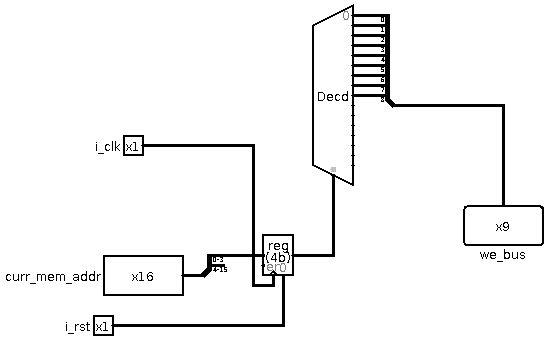
\includegraphics[scale=0.5]{reg_enabler.png}
    \caption[Gestore registri]{Il modulo responsabile dell'abilitazione dei registri.\label{reg_enabler}}
\end{figure}

L'altro componente del controller è un semplice process che, in corrispondenza del fronte di salita del clock, determina il registro di lavoro da abilitare
in scrittura, basandosi sul valore corrente dell'indirizzo. In questo modo, il registro corretto può immediatamente acquisire il nuovo valore.

\section{Risultati sperimentali}

\subsection{Report di sintesi}
Si riportano frammenti del report di sintesi per il componente.

\lstdefinestyle{synthresport}{language={},numbers=none,basicstyle={\tiny\ttfamily},breaklines}

\begin{minipage}{\linewidth}
    \lstinputlisting[style=synthresport,firstline=42,lastline=58]{../RL1920.runs/synth_1/project_reti_logiche.vds}
    \captionof*{table}{Sintesi degli elementi sequenziali.}
\end{minipage}

\begin{minipage}{\linewidth}
    \lstinputlisting[style=synthresport,firstline=69,lastline=121]{../RL1920.runs/synth_1/project_reti_logiche.vds}
    \captionof*{table}{Statistiche dei componenti RTL.}
\end{minipage}

\begin{minipage}{\linewidth}
    \lstinputlisting[style=synthresport,firstline=241,lastline=272]{../RL1920.runs/synth_1/project_reti_logiche.vds}
    \captionof*{table}{Statistiche di utilizzo.}
\end{minipage}

\subsection{Simulazioni}
Per condurre le simulazioni in un regime simile a quello dell'ipotetico normale funzionamento, è stato creato un apposito programma di simulazione
comandabile da file. Tale apparato di testing ha reso semplice non solo eseguire più attivazioni successive con indirizzi e working-zones diverse, ma anche
la generazione automatica di test casuali per mezzo di un apposito fuzzer.

Per i dettagli riguardanti il tester e il fuzzer, si rimanda alle appendici \ref{appendix:unitest} e \ref{appendix:fuzzer}.

\subsubsection{Test case}
Sono stati progettati alcuni test per stimolare quelle che si sono ritenute essere sezioni critiche del funzionamento o valori limite di alcune variabili,
prima di procedere con il fuzzing.

\paragraph{\emph{Full-sweep}}
Questo test punta a validare il funzionamento di base dell'encoder, fornendogli in input prima tutte le basi delle working-zones, poi prendendo una zona
isolata e richiedendo la codifica di ogni suo membro.

In questo modo è stato possibile testare gli elementi aritmetici del componente e la corretta rappresentazione delle informazioni nei campi del risultato
codificato.

\paragraph{Confini delle working-zones}
Test per la verifica dell'appartenenza e della non appartenenza degli indirizzi posti ai margini delle working-zones. Si sono piazzate alcune WZ su range
di indirizzi adiacenti e non, ed è stato richiesto al componente di produrre codifiche per gli indirizzi posti ai loro estremi e immediatamente al di
fuori di essi.

In questo modo sono stati validati i comparatori paralleli e i mux di selezione.

\paragraph{Riproducibilità}
Si è richiesta la codifica dello stesso indirizzo sia in due volte consecutive, sia dopo altri test. Un test banale per una proprietà universale
fondamentale.

\paragraph{Modifica delle working-zones e reset}
Codifica, sostituzione e riorganizzazione delle working-zones, reset e successivo test di ricodifica. Alcuni indirizzi, che ricadevano al di fuori delle WZ
nell'esecuzione precedente, sono utilizzati per verificare che l'inserimento di WZ che li contengono portino effettivamente alla nuova codifica, una volta
avviata una nuova esecuzione (\emph{reset} + \emph{start}).

\paragraph{Confini della memoria}
Questo test controlla la correttezza nella rappresentazione degli indirizzi 0 e 127, sia che essi siano inclusi in working-zones terminali, sia che non lo
siano. È un ulteriore test per la validazione dei comparatori e degli altri componenti algebrici.

\paragraph{Partenza anticipata}
Si è rimosso il ciclo di stasi dopo il segnale di reset per verificare che il funzionamento risulti corretto anche sotto vincoli di tempo più stringenti di
quelli imposti nel test di riferimento.

\paragraph{Reset durante la codifica}
Test che tenta di produrre una criticità nella macchina di controllo inviando un segnale di reset durante la fase di ouput dell'indirizzo codificato (stato
\emph{WA}), verificando che ciò provochi un regolare reset.

Tale verifica è effettuata spostando una zona senza resettare la macchina e chiedendo la codifica di un indirizzo precedentemente coperto da essa. Se la
codifica cambia nella maniera attesa, il reset è avvenuto con successo.

\paragraph{Reset durante il caricamento delle zone}
Si inviano brevi segnali \emph{reset} al componente mentre questo sta procedendo al caricamento delle zone. Con un accurato timing degli impulsi, si cerca
di produrre criticità negli elementi di controllo, specialmente in quello adibito all'attivazione dei registri di lavoro. Con impulsi sia prima che dopo
il fronte di salita del clock, si verifica che tutte le zone vengano opportunamente ricaricate, sfruttando la stessa strategia del test precedente.

\subsubsection{\emph{Fuzzing}}
Il componente è stato sottoposto a varie iterazioni di fuzzing (molte migliaia), dove sia working-zones che indirizzi son stati generati casualmente.
La generazione è avvenuta  rispettando le condizioni di non sovrapposizione delle WZ, il range di indirizzi 0-127 e alcune regole di ottimizzazione
aggiuntive.

In particolare, ad ogni iterazione si visitano in ordine casuale indirizzi appartenenti ad un insieme che racchiude strettamente quelli coperti dalle
zone di lavoro, evitando inutili percorsi nello spazio d'indirizzamento che non attivano nessuna codifica speciale.

\section{Conclusioni}
Il componente risulta funzionante entro le specifiche dettate. Grazie alla memorizzazione interna delle working-zones e alla comparazione parallela, è
possibile la sua integrazione in un sistema che richieda di convertire, a ritmi non troppo elevati, un flusso di indirizzi fisici in un flusso codificato.

Durante il testing si è prestata particolare attenzione nel validare il componente ponendo limiti più stretti di quelli comunicati esplicitamente nel
documento di specifica, o implicitamente attraverso il test bench di riferimento; in particolare, si è tentato di eliminare i cicli di attesa tra le
conversioni e si sono controllati più frequentemente i segnali emessi dal componente.

Spingendosi brevemente nel dominio delle simulazioni timing, si è anche preventivamente corretto un problema di glitch sul segnale \emph{done}, filtrandolo
con un flip-flop.

\newpage

\appendix
\section{Tester unificato}
\label{appendix:unitest}
Per verificare il corretto funzionamento del componente, è stato realizzato un programma VHDL in grado di presentare all'UUT una RAM analoga a quella
fornita col test di esempio, ma i cui valori possono essere aggiornati da parte di un process di controllo, a sua volta pilotato da un file di stimoli
esterno.

Per ogni linea del file sono specificati i segnali da inviare al componente (\lstinline{tb_reset} e \lstinline{tb_start}), i valori da scrivere in RAM
(indirizzo e contenuto) e il tempo da attendere dopo ogni aggiornamento.\\
Inoltre, alcune linee speciali segnalano al tester di eseguire una verifica del risultato; in questo caso, il programma si pone in attesa del segnale di
\emph{done} e, non appena questo viene alzato, verifica che il valore presente all'indirizzo 0009 sia uguale a quello specificato sulla linea di
checkpoint. Inoltre, il risultato viene ricontrollato anche in corrispondenza dell'abbassamento di \lstinline{tb_done} per scongiurare il rischio di
riscritture accidentali dovute a malfunzionamenti dell'unità di controllo.

Poiché il programma si ferma solo in corrispondenza della fine del file, è possibile lanciare più esecuzioni, anche con working-zones diverse, all'interno
di una stessa simulazione.

Per rendere più agevole la correzione dei difetti, il tester è in grado di stampare eventuali messaggi presenti in coda alle linee dei segnali.

\pagebreak
\subsubsection{Implementazione del tester}
\lstinputlisting[firstline=22,breaklines]{../RL1920.srcs/sim_1/new/unitest.vhd}

\subsubsection{File di stimolo utilizzato}
\lstinputlisting[numbers=none,breaklines]{../tests/electrosaint.pertini.txt}
\pagebreak

\section{Fuzzer}
\label{appendix:fuzzer}
Per rendere meno probabile la presenza di difetti non rilevati attraverso i test manuali, è stato realizzato un fuzzer in grado di generare casualmente
delle working-zones e un set appropriato di indirizzi col quale testare la funzionalità del componente.

Il fuzzer è stato implementato nella forma di un semplice script Python che, dato in input un intero, restituisce in ouput un egual numero di
``test runs'', dove una test run è una serie di linee di testo nel formato utilizzato dal tester, le quali descrivono un caricamento di working-zones
seguito da molteplici richieste di codifica, ognuna seguita a sua volta dal corrispondente checkpoint.

La generazione dei test avviene rispettando le seguenti regole:
\begin{enumerate}
    \item Le working-zones non devono sovrapporsi, e lo spazio indirizzato da ciascuna deve trovarsi all'interno dell'intervallo 0-127.
    \item Gli indirizzi 0, 1, 126 e 127 devono essere sempre visitati.
    \item Per ogni zona, detta $B$ la sua base, devono essere visitati gli indirizzi dell'intervallo $[B - 2, B + 6]$.
    \item Ciascun indirizzo dev'essere visitato una sola volta.
    \item Gli indirizzi da verificare devono essere visitati in ordine casuale.
\end{enumerate}

In questo modo, è stato possibile sottoporre il componente ad un gran numero di test in maniera semiautomatica.

\pagebreak
\subsubsection{Implementazione del fuzzer}
\lstinputlisting[language=python,breaklines]{../tests/fuzz.py}

\end{document}
